\def\layersep{2.5cm}
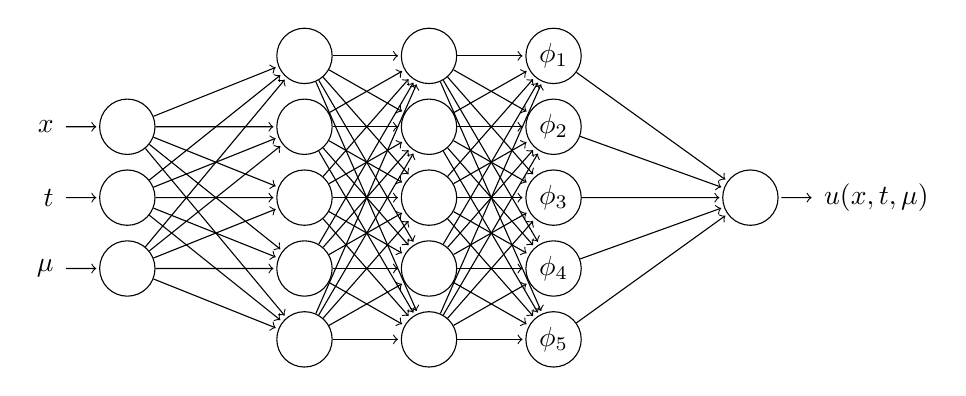
\begin{tikzpicture}[shorten >=1pt,->,draw=black!100, node distance=\layersep,scale=0.9]
    \tikzstyle{every pin edge}=[<-,shorten <=1pt]
    \tikzstyle{neuron}=[circle,fill=black!25,minimum size=20pt,inner sep=0pt]
    \tikzstyle{input neuron}=[neuron, fill=gray!0,draw=black];
    \tikzstyle{output neuron}=[neuron, fill=gray!0,draw=black];
    \tikzstyle{hidden neuron}=[neuron, fill=gray!0,draw=black];
    \tikzstyle{hidden neuron b}=[neuron, fill=gray!0,draw=black];
    \tikzstyle{hidden neuron c}=[neuron, fill=gray!0,draw=black];
    \tikzstyle{annot} = [text width=4em, text centered]

    % Draw the input layer nodes
    %\foreach \name / \y in {1,...,3}
    % This is the same as writing \foreach \name / \y in {1/1,2/2,3/3,4/4}
    %\node[input neuron, pin=left:$\text{feature }{\y}$] (I-\name) at (0,-\y) {};
    \path[yshift=0.5cm]
    node[input neuron, pin=left:${\boldsymbol x}$] (I-1) at (0,-2) {};
    \path[yshift=0.5cm]
    node[input neuron, pin=left:$t$] (I-2) at (0,-3) {};
    \path[yshift=0.5cm]
    node[input neuron, pin=left:$\boldsymbol \mu$] (I-3) at (0,-4) {};

    % Draw the hidden layer nodes
    \foreach \name / \y in {1,...,5}
        \path[yshift=0.5cm]
            node[hidden neuron] (H-\name) at (\layersep,-\y cm) {};

    \foreach \name / \y in {1,...,5}
        \path[yshift=0.5cm]
            node[hidden neuron b] (H2-\name) at (\layersep +50,-\y cm) {};

    \foreach \name / \y in {1,...,5}
        \path[yshift=0.5cm]
            node[hidden neuron c] (H3-\name) at (\layersep +100,-\y cm) {};

    % Draw the output layer node
    \path[yshift=0.5cm]
    node[output neuron,pin={[pin edge={->}]right:$\boldsymbol u(\boldsymbol x,t,\boldsymbol \mu)$}, right of=H3-3] (O) {};

    % Connect every node in the input layer with every node in the
    % hidden layer.
    \foreach \source in {1,...,3}
        \foreach \dest in {1,...,5}
            \path (I-\source) edge (H-\dest);


    \foreach \source in {1,...,5}
        \foreach \dest in {1,...,5}
            \path (H-\source) edge (H2-\dest);

    \foreach \source in {1,...,5}
        \foreach \dest in {1,...,5}
            \path (H2-\source) edge (H3-\dest);

    % Connect every node in the hidden layer with the output layer
    \foreach \source in {1,...,5}
        \path (H3-\source) edge (O);

    % Annotate the layers
    %\node[annot,above of=H-1, node distance=1cm] (hl) {Hidden layer};
    \node[annot,above of=H3-1, node distance=0cm] (h2) {$\boldsymbol \phi_1$};
    \node[annot,above of=H3-2, node distance=0cm] (h3) {$\boldsymbol \phi_2$};
    \node[annot,above of=H3-3, node distance=0cm] (h4) {$\boldsymbol \phi_3$};
    \node[annot,above of=H3-4, node distance=0cm] (h5) {$\boldsymbol \phi_4$};
    \node[annot,above of=H3-5, node distance=0cm] (h6) {$\boldsymbol \phi_5$};
    %\node[annot,left of=hl] {Input layer};
    %\node[annot,right of=hl] {Output layer};
\end{tikzpicture}
